\chapter{State of the Art} \chaplabel{state-of-the-art}

In diesem Kapitel gebe ich einen Überblick über Projekte, welche ähnliche
Zielsetzungen haben, sowie über publizierte Forschungsarbeiten zu verwandten
Themen.

\section{Sensorhandschuhe}

Verschiedene Arten von Sensorhandschuhen und sogenannten ,,smart gloves''
finden in der Forschung Anwendung. Die einfachsten davon enthalten Taster oder
leitfähige Flächen~\cite{web:keyglove}, um direkte Eingaben zu ermöglichen
(vgl. \figref{keyglove}).  Andere basieren auf Flex- oder Stretch-Sensoren
\citep{glove-ole}, um den Biegungsgrad der Finger, teilweise auch der einzelnen
Fingerglieder zu messen.  In \subsecref{flex} gehe ich darauf ein, warum wir
diesen Ansatz nicht verfolgt haben. Eine Übersicht über diese frühen Ansätze
bieten \citet{dipietro-gloves-survey}.

\begin{figure}
    \centering
    \fbox{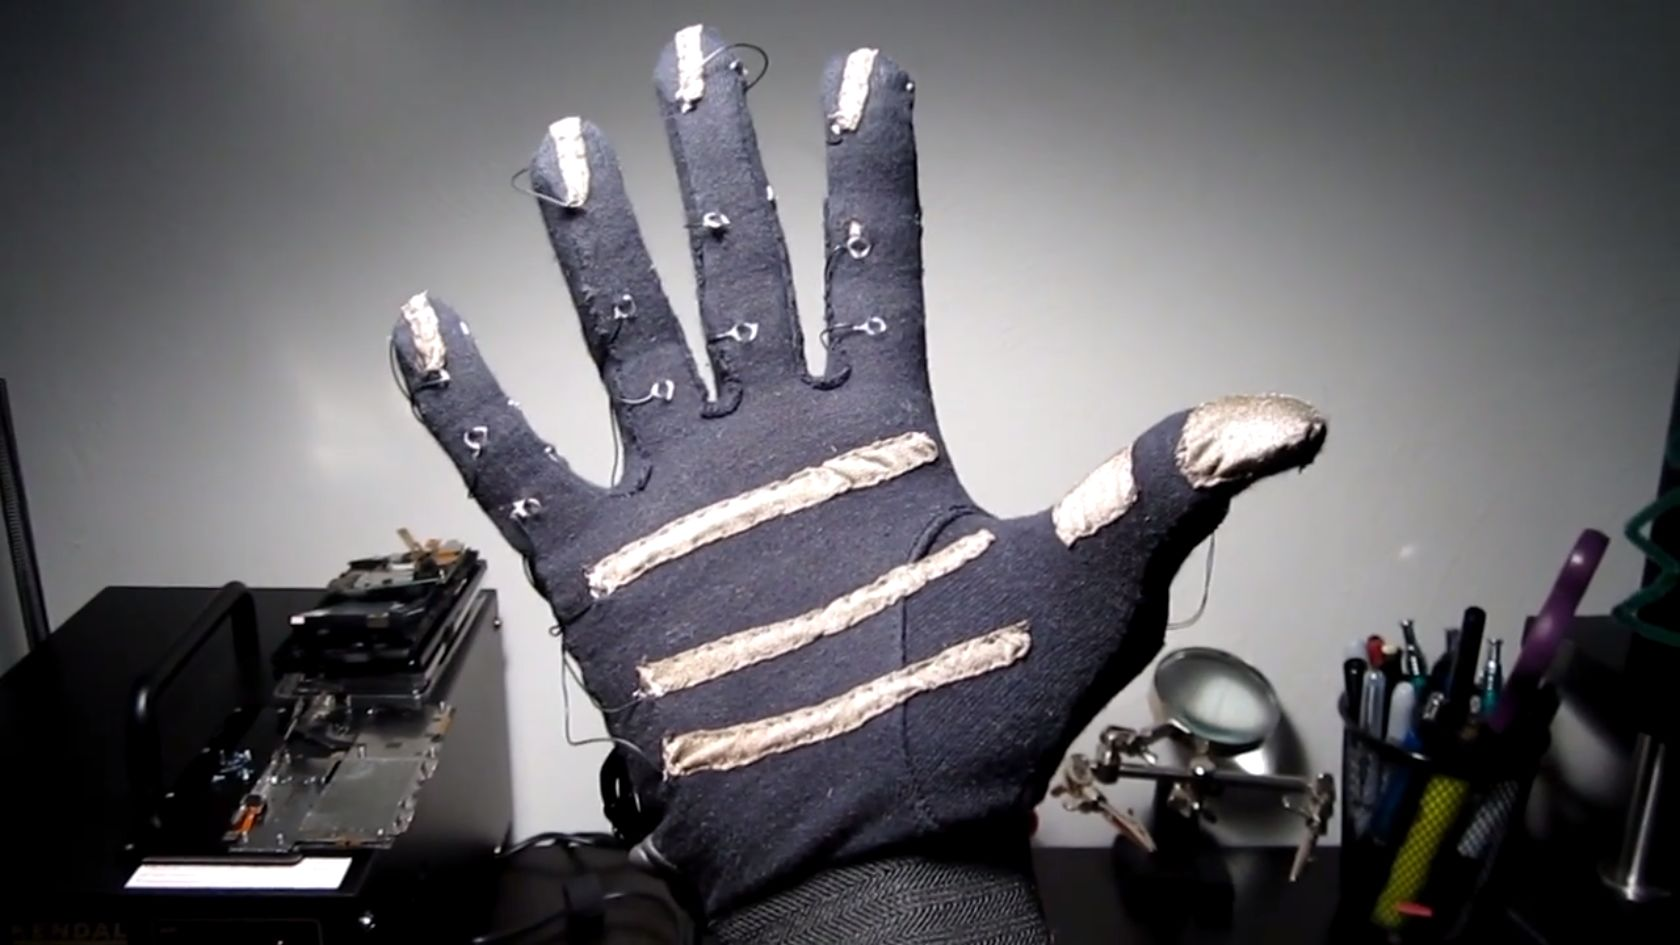
\includegraphics[width=0.8\textwidth]{../common/images/keyglove}}
    \imagesource{https://vimeo.com/23269969}
    \caption[Der ,,Keyglove''~\cite{web:keyglove}]{Der ,,Keyglove'' ist ein tragbares Gerät zur Tastatureingabe, basierend auf leitfähigen Kontaktpunkten~\cite{web:keyglove}.}
    \figlabel{keyglove}
\end{figure}

Die Verwendung von IMUs\footnote{Inertial measurement units; in \subsecref{imu}
erläutere ich deren Aufbau und Funktionsweise.} in Sensorhandschuhen ist
relativ neu (in der Übersicht von 2008 finden sich noch keine Projekte mit
IMUs), sie sind besonders in der medizinischen Forschung präsent.
Sensorhandschuhe können hier zum Beispiel Ärzte unterstützen, indem sie die
Handbewegungen von Patienten während der Rehabilitation nach Handverletzungen
aufzeichnen~\citep{glove-medical-imu}. An den Bewegungswerten sind Muster zu
erkennen, welche auf den Fortschritt der Heilung schließen lassen.
Sensorhandschuhe werden ebenso zu Untersuchungen in Studien der
Parkinson-Krankheit eingesetzt \citep{cavallo-senshand-parkinsons}.

Andere Projekte erweitern den Sensorhandschuh um Komponenten für Feedback an
den Benutzer, hauptsächlich visuelles Feedback durch LEDs und haptisches
Feedback durch \emph{vibro-tactile stimulators}. Die
,,InerTouchHand'' \citep{inertouchhand} zum Beispiel wurde zur Forschung der
\emph{human-machine interaction} entwickelt, Zielanwendung ist die Steuerung
einer menschenähnlichen Roboterhand. Auch dieses Projekt verwendet IMUs zur
Messung der Handhaltung.

Es gibt ferner kommerzielle Produkte, welche ähnliche Technologien verwenden.
Angetrieben wird die Entwicklung dieser Produkte meist von der
Computerspielebranche. Ein populäres Produkt ist die Nintendo
Wii\textsuperscript{\texttrademark} Spielekonsole, in deren Fernbedienung ein
Accelerometer verbaut ist~\cite{web:wii-mote-guts}, um innovative Steuerung von
Spielen zu ermöglichen.  Auch in der Virtual-Reality Branche wird viel mit
diesen Sensoren gearbeitet. So enthalten zum Beispiel die Brille und
Hand-Controller des HTC Vive\textsuperscript{\textregistered} VR-Systems die
\productname{InvenSense MPU-6500} (Accelerometer und
Gyroskop)~\cite{web:vive-teardown}.

Ein tatsächlicher Sensorhandschuh ist der \productname{Hi5 VR Glove} von Noitom
Ltd, ein kürzlich vorgestelltes Produkt. Es wird als ,,wireless consumer glove
designed for virtual reality headsets''~\cite{web:hi5vrglove} beworben, ist
jedoch noch nicht auf dem Markt erhältlich. Der Handschuh enthält, genau wie
unser Prototyp, sechs IMUs. Eine Software, die Tastatur\-emulation
durchführt, wird allerdings nicht erwähnt.

\section{Alternative Texteingabegeräte}

Sehr ähnlich zu unserem Projekt war das Produkt
\citetitle{web:gest}~\cite{web:gest}.  Hierbei handelte es sich um ein tragbares
Gerät, welches an der Hand und 4 Fingern befestigt wurde (vgl. \figref{gest}) und ebenfalls IMUs
enthielt.  Das Produkt wurde im November 2015 mit einer
Kickstarter-Kampagne\footnote{\url{https://www.kickstarter.com/projects/asdffilms/gest-work-with-your-hands}}
finanziert, und sollte ein General-Purpose-Device zur Interaktion mit Computern
werden. Die Entwickler stellten das Gerät auch, anders als der Hersteller des
Hi5 VR Glove, für die Verwendung als Tastatur vor, und zeigten beispielhaft in
einem Werbevideo\footnote{\url{https://vimeo.com/143556093}} diese
Funktionalität.  Sie spezifizierten leider nicht öffentlich wie die Erkennung
durchgeführt wurde, und das Projekt wurde aufgrund mangelnder Investitionen
Mitte 2016 eingestellt.

Eine weitere zu unserem Projekt sehr ähnliche Arbeit ist
\citetitle{nasa-joystick-keyboard}~\citep{nasa-joystick-keyboard}. Damit wurde
bereits 2003 ein Ansatz entwickelt, um mithilfe von EMG-Messungen Joysticks und
Tastaturen zu emulieren. Für letztere befestigten die Autoren 8 EMG-Elektroden
am Unterarm des Probanden, zeichneten Bewegungen auf und lernten, die Muster
mit Hidden Markov Models zu erkennen.  In ihren Versuchen stellten sie Probleme
bei der Verwendung von EMG-Eletroden fest. Grundsätzlich war die Leistung des
Systems von der Position der Elektroden, Schweiß, trockener Haut, Tragezeit
sowie der allgemeinen Tagesform des Probanden abhängig. Für die Steuerung eines
Flugzeuges im Simulator waren die 4 erkannten Joystick-Gesten (links, rechts,
auf, ab) ausreichend akkurat. Das Tippen auf dem Ziffernblock einer Tastatur
klappte ebenfalls mit etwa 80\% Genauigkeit, wenn das Modell am Tag der
Verwendung trainiert wurde, und die Elektroden somit identisch platziert waren.

\vfill
\begin{figure}[h]
    \centering
    \fbox{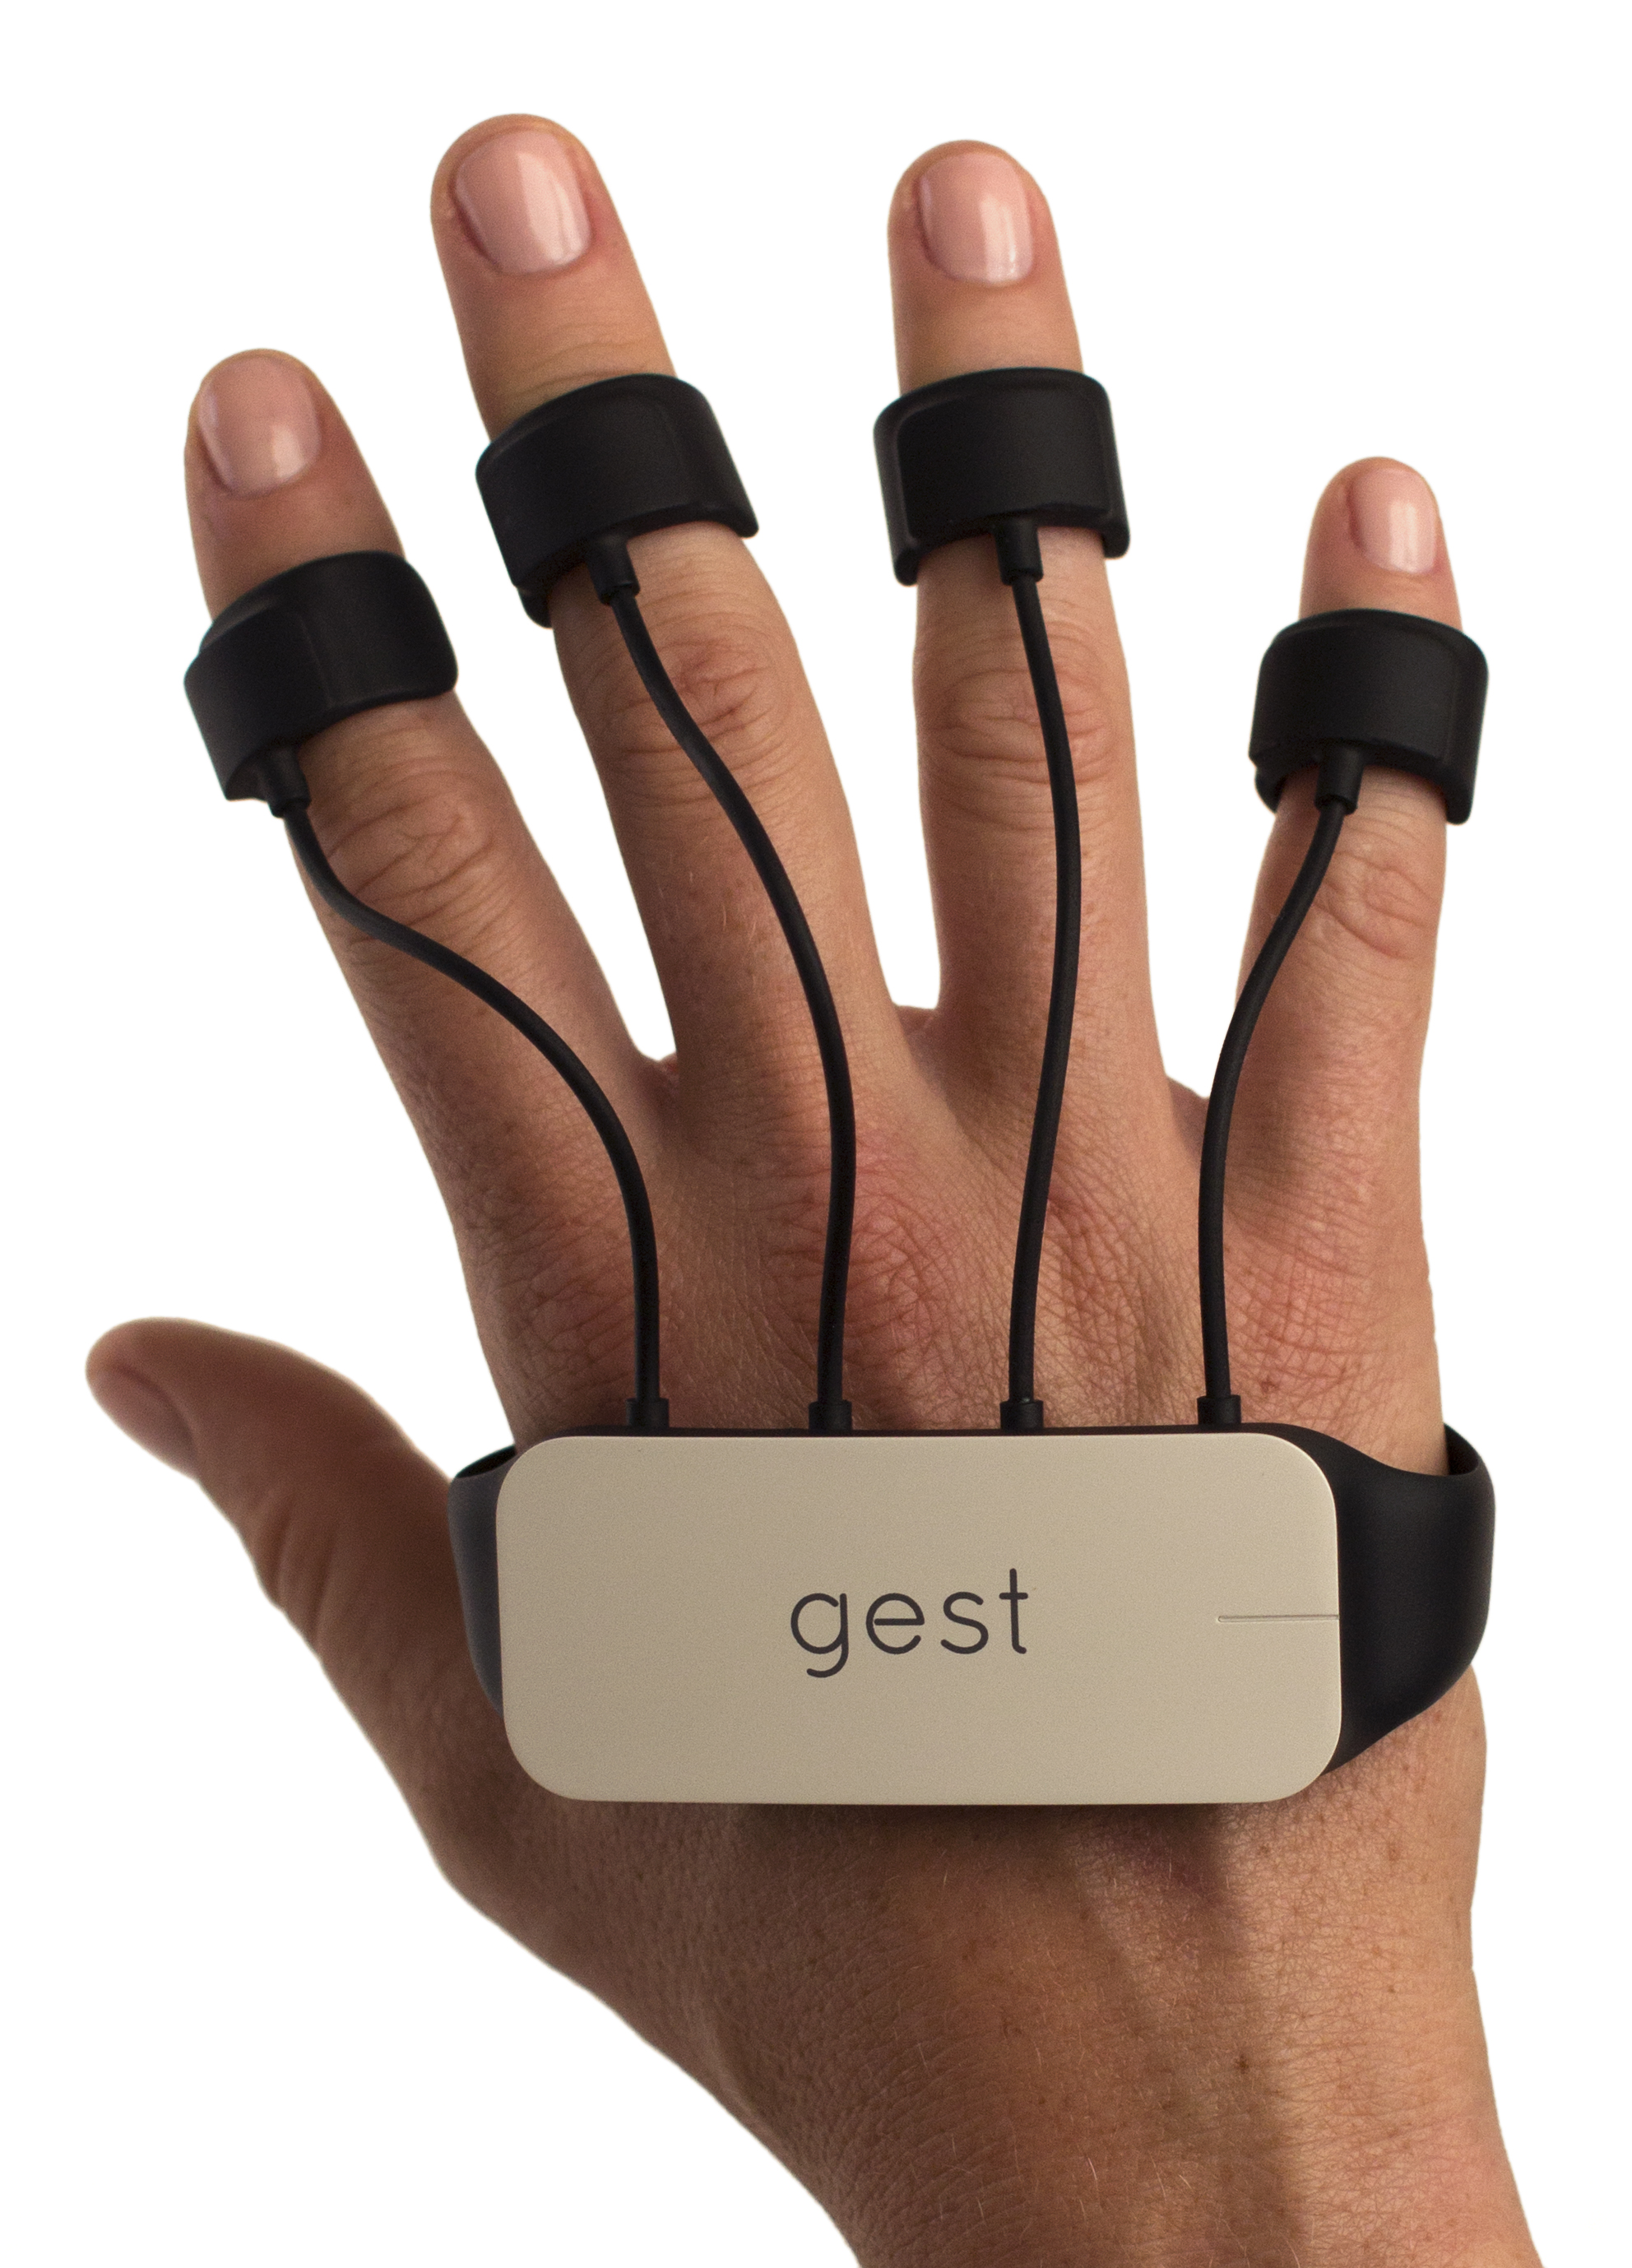
\includegraphics[height=8cm]{../common/images/gest-white}}
    \imagesource{https://gest.totemapp.com/company}
    \caption[Gest (Werbebild)~\cite{web:gest}]{Gest sollte ein tragbares
    General-Purpose-Device zur Interaktion mit Computern werden. Dazu war
    ebenfalls die Umsetzung einer virtuellen Tastatur angekündigt. Das Projekt
    wurde jedoch eingestellt. (Werbebild)}
    \figlabel{gest}
\end{figure}


\section{Visuelles Hand-Tracking}\seclabel{visuelles-system}

Forscher von Microsoft Research haben einen Algorithmus entwickelt, um
Handposen aus Kamerabildern mit Tiefeninformation zu
extrahieren \citep{microsoft-hand-tracking}. Verwendet wird hierbei eine
Microsoft Kinect. Die rekonstruierte Handpose wird für die Manipulation
virtueller 3D-Objekte benutzt.

,,\citetitle{ellithorpe-kinect-typing}'' \citep{ellithorpe-kinect-typing}
verwendet ebenfalls eine Kinect, allerdings um getippte Wörter auf einer
Tastatur zu erkennen.  Hierfür kommen verschiedene Bildverarbeitungsschritte
zur Vorverarbeitung und \fremdwort{Support Vector Machines} zur Klassifikation
zum Einsatz. Diese erlangten eine erstaunliche Genauigkeit von über 80\% auf
einem Datensatz mit 114 verschiedenen Wörtern.

\section{Maschinelles Lernen und IMUs}

Ein weiterer relevanter Forschungsbereich ist die \emph{Human Activity
Recognition} (HAR). Das Ziel der HAR ist es, menschliche Aktivitäten aus
Sensordaten zu erkennen. Hierfür kommen zahlreiche unterschiedliche Sensoren
zum Einsatz, darunter Accelerometer, Gyroskope und Magnetometer aber zum
Beispiel auch GPS, Mikrofone, Drucksensoren, Kameras und Thermometer. Mithilfe
von Methoden des maschinellen Lernens wird versucht, zwischen alltäglichen
Aktionen zu unterscheiden, etwa dem Gehen, Stehen, Sitzen, Liegen, aber auch
Öffnen von Türen oder Schubladen sowie die Manipulation kleinerer Objekte
\citep{lara-har}. Verwendet werden dafür seit längerem Ansätze des maschinellen
Lernens. Inzwischen kommen unter anderem auch \fremdwort{Convolutional Neural
Networks} (CNNs) zum Einsatz \citep{dense_labeling}, welche wir auch in diesem
Projekt verwenden.

% * Traditionell / Kalman-Filter :(
% * Madgwick :)

% Madgwick:
% * mega spannend
% * konvergiert langsamer (small gain)
% * konfigurierbar, dann schneller
% * aber man will so langsam wie möglich da größerer gain -> mehr noise
% * vielleicht kaum nötig wenn gyro nicht clippt :)
% * also mal als alternative probieren mit 2000 deg/s
% * selbstkalibrierend (gyro bias)
% * kein problem mit heading-fehlern wenn korrigiert durch gravity während acceleration
